\documentclass[a4paper,12pt]{report}

% --- CẤU HÌNH TIẾNG VIỆT & FONT ---
\usepackage[utf8]{inputenc}
\usepackage[T5]{fontenc} % Bắt buộc cho tiếng Việt
\usepackage[vietnamese]{babel}
\usepackage{lmodern}
\usepackage{mathptmx} % Font giống Times New Roman, gọn gàng hơn cho báo cáo

% --- CÁC GÓI HỖ TRỢ ---
\usepackage{geometry}
\usepackage{amsmath, amssymb, amsfonts}
\usepackage{graphicx}
\graphicspath{{../figures/}}
\usepackage{svg} % Hỗ trợ file SVG
\usepackage{booktabs}
\usepackage{float}
\usepackage{enumitem}
\usepackage{cite}
\usepackage[hyphens]{url} % Hỗ trợ URL trong bibliography với khả năng xuống hàng
\usepackage{xcolor}
\usepackage{titlesec}
\usepackage{caption}
\usepackage[breaklinks=true,hidelinks]{hyperref} % Cho phép URL xuống hàng

% --- CẤU HÌNH URL ---
\def\UrlBreaks{\do\/\do\-\do\.\do\=\do\?\do\&} % Cho phép URL break tại các ký tự này
\urlstyle{same} % Giữ nguyên font như văn bản

% --- CẤU HÌNH TRANG ---
\geometry{left=2.5cm, right=2.5cm, top=2.5cm, bottom=2.5cm}
\linespread{1.2} % Giãn dòng 1.2 cho thoáng, dễ đọc
\setlength{\parskip}{6pt} % Khoảng cách giữa các đoạn văn

% Dùng section làm cấp cao nhất trong lớp report (tránh đánh số 0.x)
\renewcommand{\thesection}{\arabic{section}}

% Nạp các chỉ số thống kê được sinh tự động từ pipeline EDA
\input{eda_stats.tex}

\begin{document}

% --- TRANG BÌA ---
\begin{titlepage}
    \centering
    
    % Logo trường (Nếu bạn có file logo.png thì bỏ comment dòng dưới)
    % 
\includegraphics[width=0.25\textwidth]{logo.png} 
    \vspace{0.5cm}
    
    % Tên trường
    {\large \textbf{ĐẠI HỌC QUỐC GIA THÀNH PHỐ HỒ CHÍ MINH}}\\
    {\large \textbf{TRƯỜNG ĐẠI HỌC KHOA HỌC TỰ NHIÊN}}\\
    
    \vspace{0.3cm}
    \rule{0.6\textwidth}{0.5pt}
    \vspace{1cm}
    
    % Môn học
    {\Large \textbf{BÁO CÁO MÔN HỌC}}\\
    \vspace{0.3cm}
    {\LARGE \textbf{THỊ GIÁC MÁY TÍNH}}
    
    \vspace{2cm}

    
\begin{figure}[H]
    \centering
    % Đảm bảo bạn có file architecture.png trong thư mục dự án
    
\includegraphics[width=0.3\linewidth]{logo.png} 
\end{figure}
    
    
    % Đề tài
    \begin{minipage}{0.9\textwidth}
        \centering
        {\LARGE \textbf{PHÂN TÍCH THỐNG KÊ CÁC TẬP DỮ LIỆU MNIST}}
    \end{minipage}

    \vfill

    \vspace{1cm}
    
    \begin{minipage}{\textwidth}
        \centering
        {\large \textbf{Giảng viên hướng dẫn:}}
        \vspace{0.3cm}
        {\large {TS. Võ Hoài Việt}}
    \end{minipage}
    
    % Thông tin sinh viên và giảng viên
    \begin{minipage}{\textwidth}
        \centering
        {\large \textbf{Sinh viên thực hiện:}}\\
        \vspace{0.3cm}
        {Lê Anh Duy (23127011)}
    \end{minipage}
    
    \vspace{1.5cm}
    
    % Thời gian
    {\large Thành phố Hồ Chí Minh, \today}
    
\end{titlepage}

% --- MỤC LỤC ---
\newpage
\tableofcontents
\newpage

\section{Giới thiệu}
\subsection{Mục tiêu}
Bài toán đặt ra là phân loại ảnh xám 28$\times$28 thuộc ba miền dữ liệu (Digit MNIST, Fashion MNIST, PneumoniaMNIST) bằng mô hình ANN cơ bản, sau đó đề xuất các cải tiến và so sánh hiệu quả.

Các Notebook thực nghiệm: \url{https://github.com/Le-Anh-Duy/CV-HOMEWORK-2-Mnist-EDA/tree/main/notebooks}.

\subsection{Ba bộ dữ liệu}
\begin{itemize}
    \item \textbf{Digit MNIST:} 10 lớp chữ số viết tay.
    \item \textbf{Fashion MNIST:} 10 lớp trang phục.
    \item \textbf{PneumoniaMNIST:} 2 lớp (Normal/Pneumonia) ảnh X-quang ngực.
\end{itemize}

\subsection{ANN là gì và vì sao chọn ANN}
ANN (Artificial Neural Network) là mô hình truyền thẳng nhiều lớp (MLP) ánh xạ vector đầu vào thành nhãn lớp. ANN đơn giản, dễ huấn luyện, cho phép tạo baseline rõ ràng để so sánh các cải tiến về đặc trưng, dữ liệu và tối ưu hóa.

\section{Dữ liệu và tiền xử lý}
\subsection{Mô tả dữ liệu}
Bảng \ref{tab:raw-dataset-summary} tóm tắt kích thước và số lượng mẫu gốc của ba tập dữ liệu.


\begin{table}[H]
    \centering
    \caption{Tổng quan thông số gốc của các tập dữ liệu (trước chuẩn hóa)}
    \label{tab:raw-dataset-summary}
    \begin{tabular}{lrrrrl}
        \toprule
        \textbf{Dataset} & \textbf{Train} & \textbf{Test} & \textbf{Classes} & \textbf{Size} & \textbf{Value range} \\
        \midrule
        Digit MNIST & 60000 & 10000 & 10 & 28$\times$28 & [0,255] \\
        Fashion MNIST & 60000 & 10000 & 10 & 28$\times$28 & [0,255] \\
        PneumoniaMNIST & 4708 & 624 & 2 & 28$\times$28 & [0,255] \\
        \bottomrule
    \end{tabular}
\end{table}

\subsection{Tiền xử lý}
\begin{itemize}
    \item Chuẩn hóa điểm ảnh về $[0,1]$ bằng cách chia 255.
    \item Làm phẳng ảnh 28$\times$28 thành vector 784 chiều để đưa vào ANN.
    \item Dùng split train/test gốc của từng tập; không tách validation cho baseline (các cải tiến có dùng tập validation nội bộ khi cần).
\end{itemize}

\subsection{Insight từ EDA}
\begin{itemize}
    \item Digit và Fashion MNIST tương đối cân bằng lớp.
    \item PneumoniaMNIST mất cân bằng mạnh giữa hai lớp, gây thiên lệch dự đoán.
    \item Tín hiệu Pneumonia thiên về \textit{texture} hơn \textit{shape}; độ biến thiên nội bộ cao.
\end{itemize}

\subsection{Minh họa dữ liệu}
\begin{figure}[H]
    \centering
    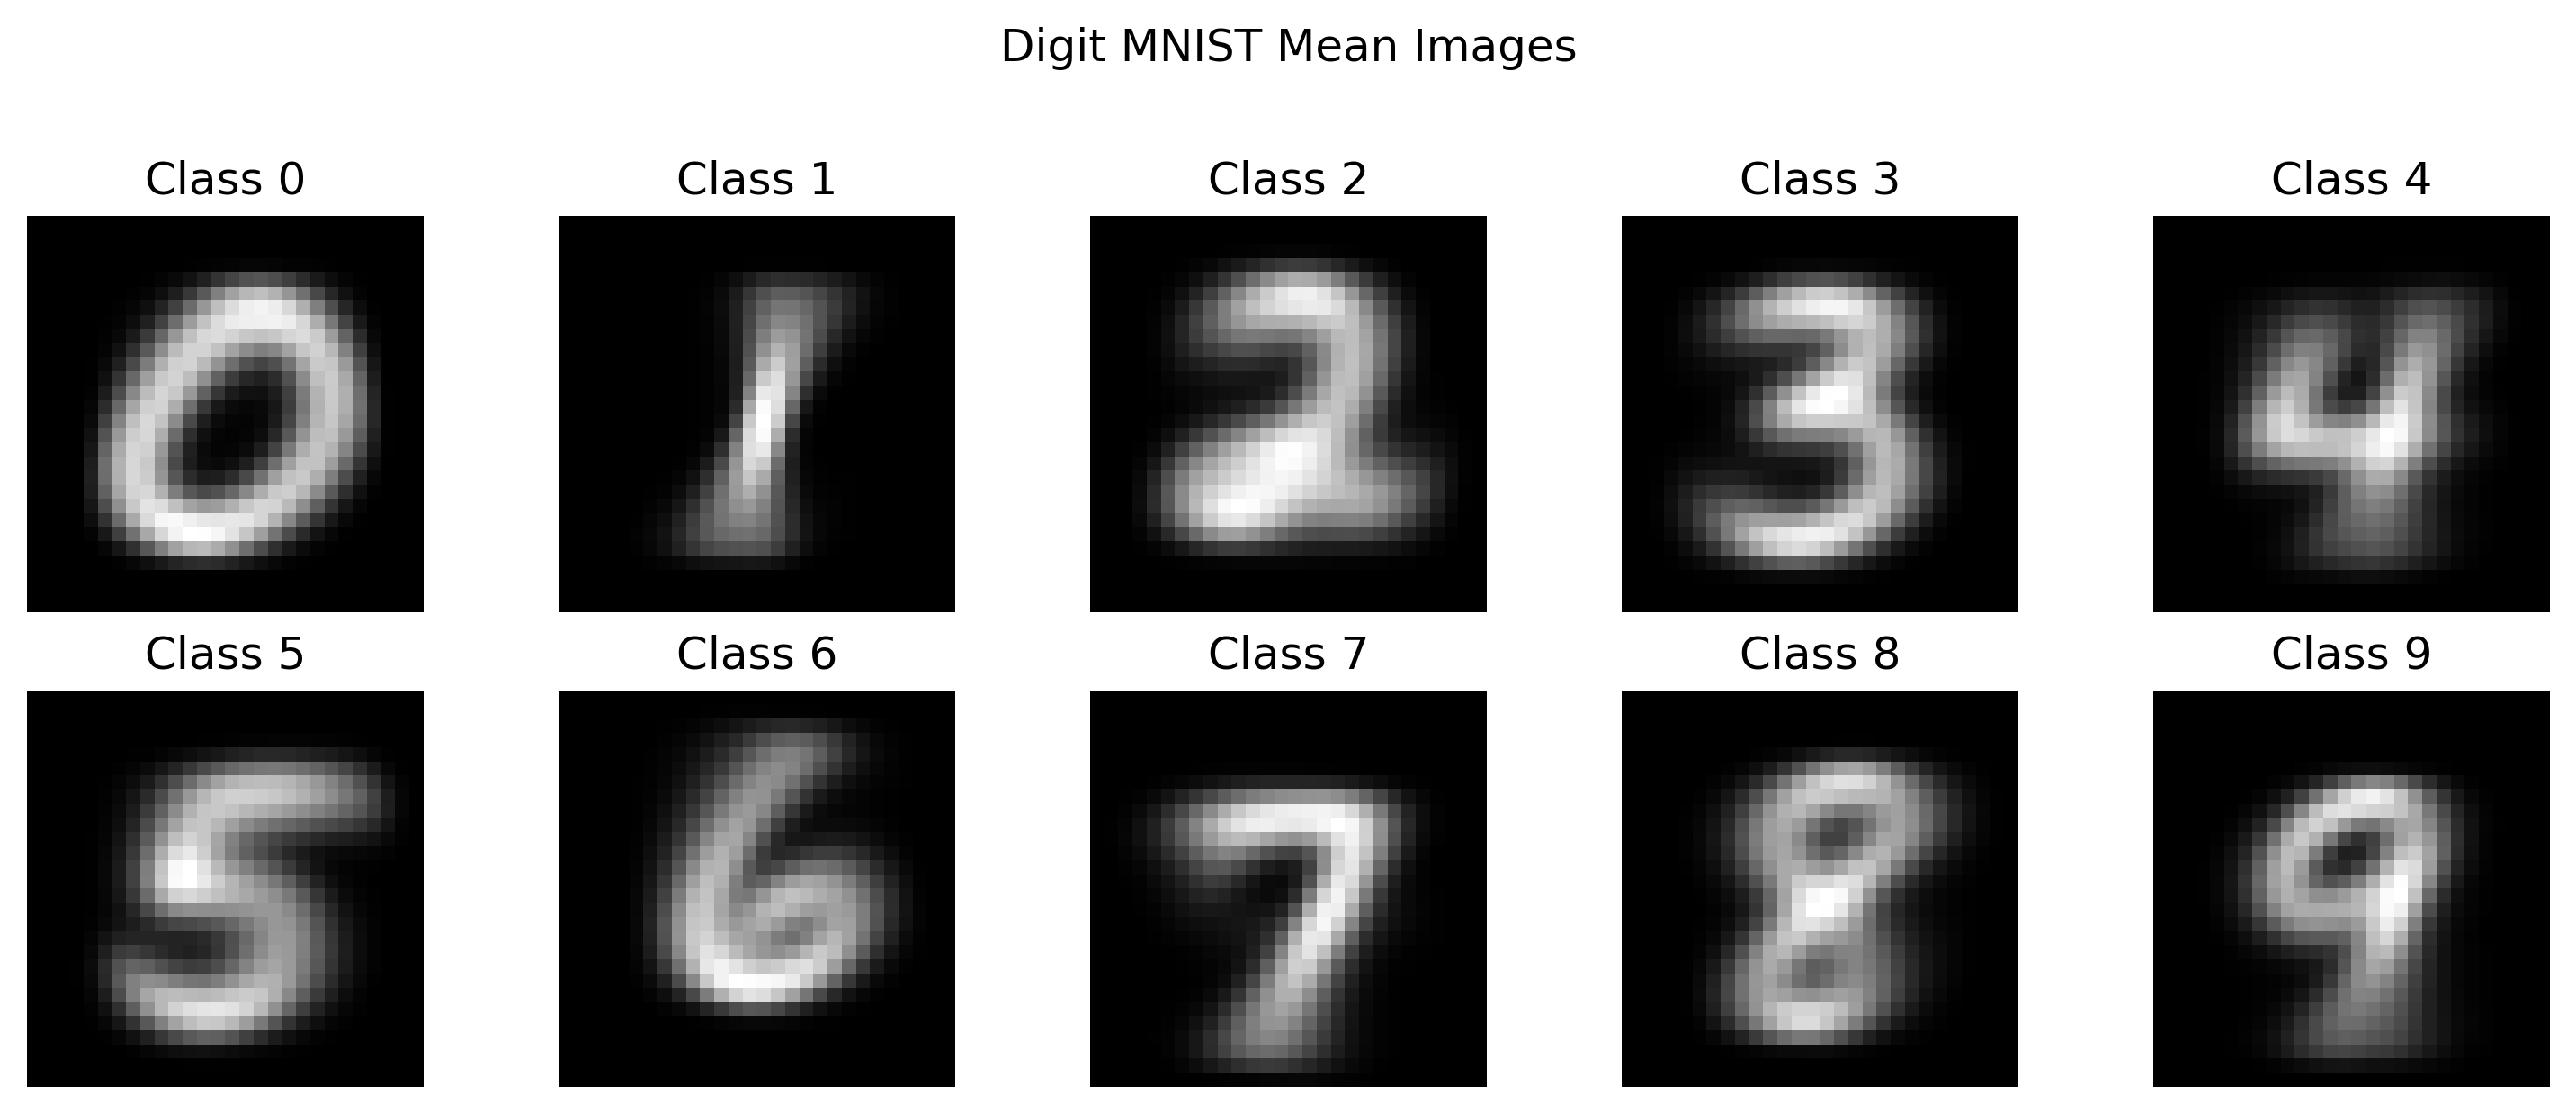
\includegraphics[width=0.28\linewidth]{mean_digit.png}
    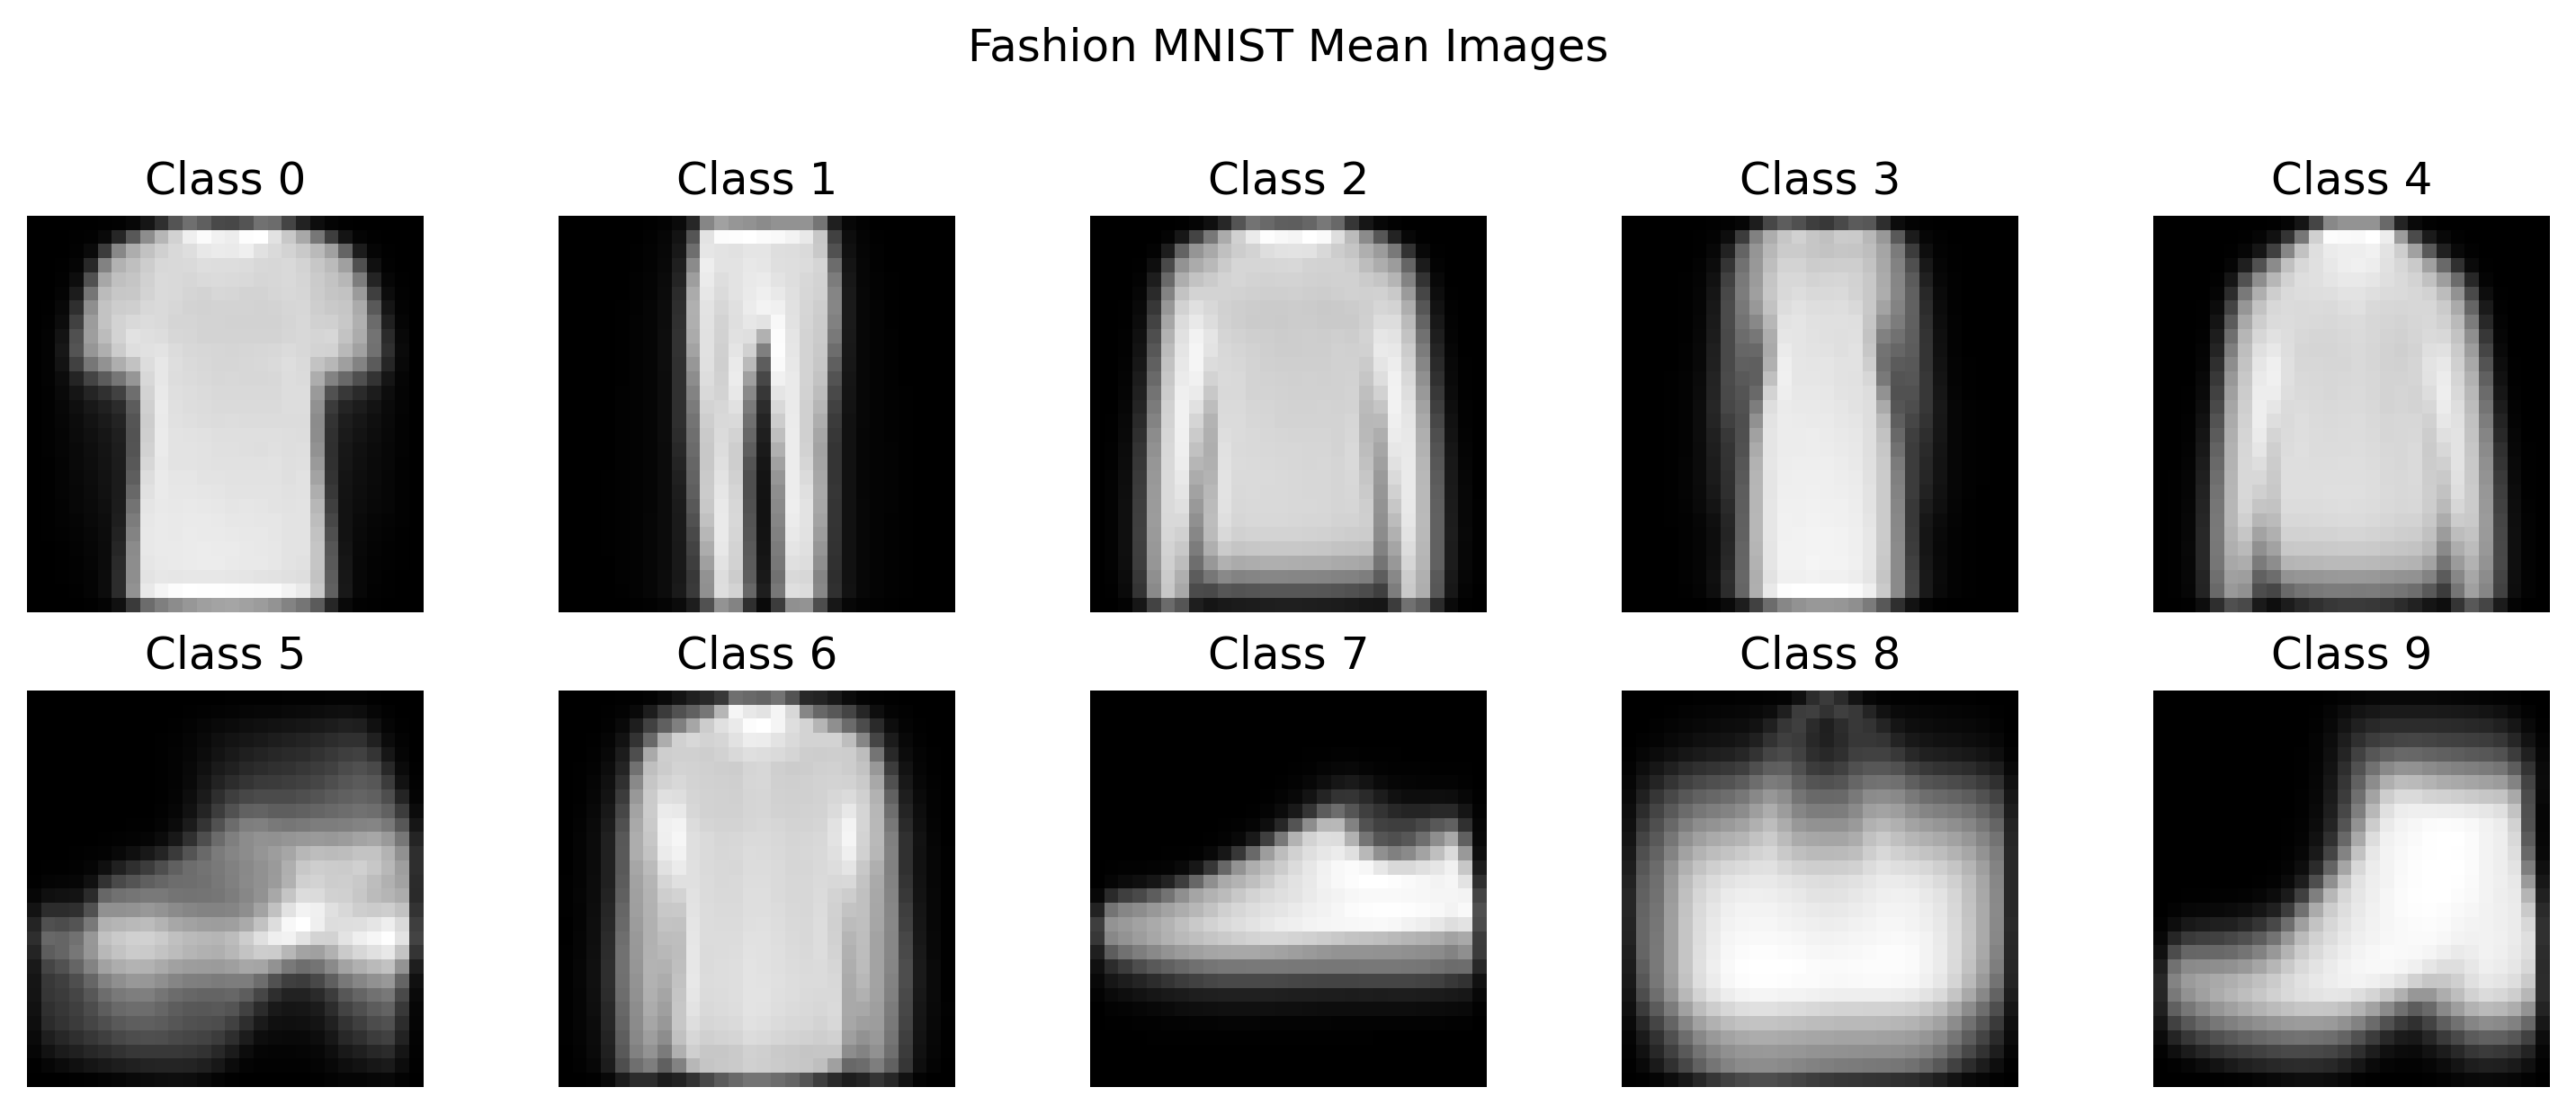
\includegraphics[width=0.28\linewidth]{mean_fashion.png}
    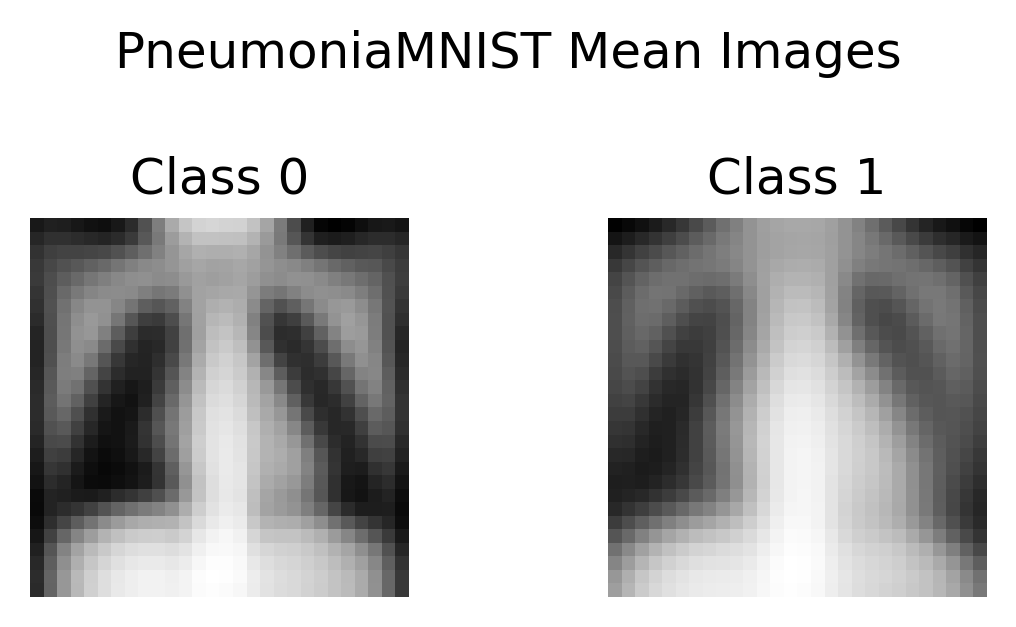
\includegraphics[width=0.28\linewidth]{mean_pneumonia.png}
    \caption{Ảnh trung bình của từng miền dữ liệu (Digit/Fashion/Pneumonia)}
    \label{fig:mean-samples}
\end{figure}

\begin{figure}[H]
    \centering
    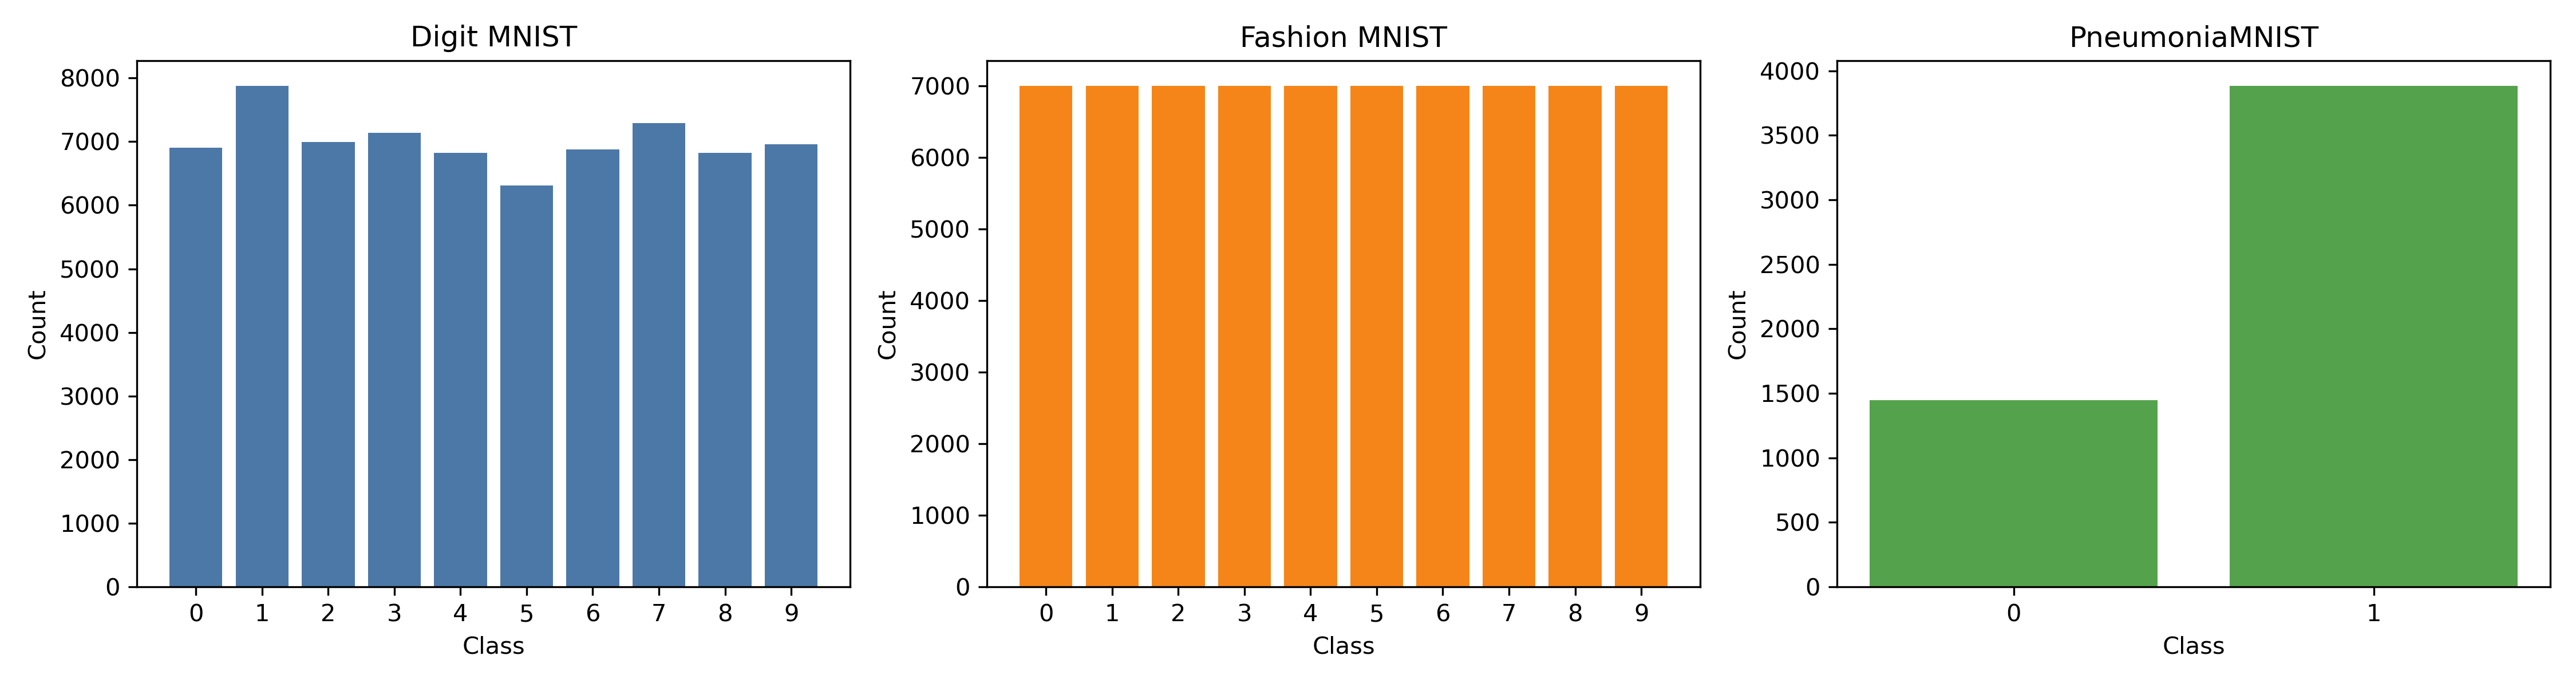
\includegraphics[width=0.65\linewidth]{label_distribution.png}
    \caption{Phân bố nhãn của ba tập dữ liệu}
    \label{fig:label-distribution}
\end{figure}

\section{Mô hình baseline}
\subsection{Kiến trúc}
ANN hai tầng ẩn: 784 $\rightarrow$ 256 $\rightarrow$ 128 $\rightarrow$ $C$ (với $C=10$ cho Digit/Fashion và $C=2$ cho Pneumonia).

\subsection{Activation}
Sử dụng ReLU ở các tầng ẩn, tầng cuối là tuyến tính (logits).

\subsection{Loss và Optimizer}
\begin{itemize}
    \item Loss: \texttt{CrossEntropyLoss}.
    \item Optimizer: Adam.
\end{itemize}

\subsection{Hyperparameters}
Epochs từ 100-600, learning rate = 0.001, huấn luyện theo full-batch (flatten toàn bộ tập huấn luyện trước khi tối ưu).

\section{Kết quả baseline}
\subsection{Bảng kết quả}
\begin{table}[H]
    \centering
    \caption{Kết quả baseline (test set)}
    \label{tab:baseline-metrics}
    \begin{tabular}{lrrrr}
        \toprule
        \textbf{Dataset} & \textbf{Accuracy} & \textbf{F1} & \textbf{Precision} & \textbf{Recall} \\
        \midrule
        Digit MNIST & 0.9438 & 0.9437 & 0.9437 & 0.9438 \\
        Fashion MNIST & 0.8443 & 0.8425 & 0.8429 & 0.8443 \\
        PneumoniaMNIST & 0.8878 & 0.8883 & 0.8896 & 0.8878 \\
        \bottomrule
    \end{tabular}
\end{table}

\subsection{Nhận xét}
Digit MNIST đạt tốt nhất; Fashion khó hơn do hình dạng đa dạng và chồng lấn giữa các lớp. PneumoniaMNIST có độ lệch lớp nên cần theo dõi đồng thời Precision/Recall thay vì chỉ Accuracy.

\section{Các cải tiến theo từng bộ dữ liệu}
\subsection{Digit MNIST}
\textbf{Cải tiến 1: HOG (feature engineering)}
\begin{itemize}
    \item Cấu hình HOG: cell 4$\times$4, block 8$\times$8, stride 4$\times$4, 9 bins; vector đặc trưng 1296 chiều.\footnote{OpenCV HOGDescriptor: \url{https://docs.opencv.org/4.x/d5/d33/structcv_1_1HOGDescriptor.html}}
    \item Kết quả: Accuracy 0.9808 (F1/Precision/Recall = 0.9808).
\end{itemize}

\textbf{Cải tiến 2: Augmentation + BatchNorm trên HOG}
\begin{itemize}
    \item Augmentation: RandomRotation $\pm10^{\circ}$, RandomAffine (translate 0.1), RandomAffine (scale 0.9--1.1).
    \item Huấn luyện batch (batch size 8192) với ANN 2 tầng ẩn, có batch norm.
    \item Kết quả tốt nhất: Accuracy 0.9939 (F1/Precision/Recall = 0.9939).
\end{itemize}

\textbf{Quan sát lỗi còn lại}
Mặc dù Accuracy đạt xấp xỉ 99\%, vẫn còn một số ảnh bị phân loại sai. Notebook clean đã trực quan hóa các mẫu sai (true vs. predicted) để minh họa các trường hợp khó, thường là chữ số viết tay bị nhiễu hoặc nét mờ.

\begin{figure}[H]
    \centering
    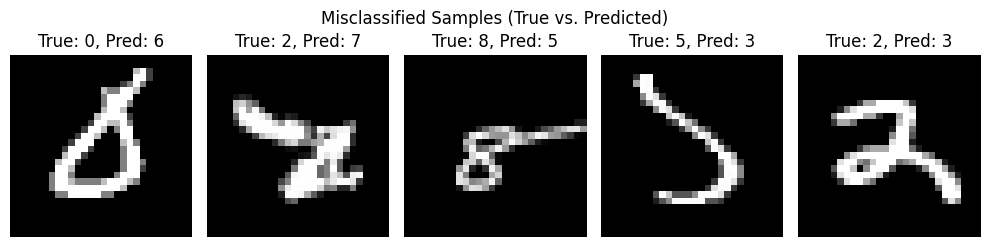
\includegraphics[width=0.7\linewidth]{ann_digit_missclassify.png}
    \caption{Các mẫu Digit MNIST bị phân loại sai (true vs. predicted)}
    \label{fig:digit-misclassified}
\end{figure}

\begin{figure}[H]
    \centering
    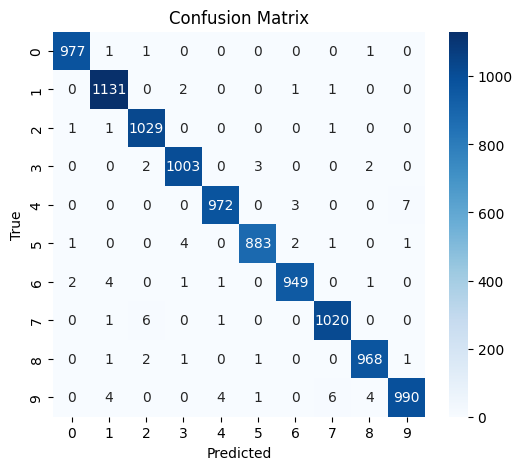
\includegraphics[width=0.55\linewidth]{ann_confusion_matrix_best_digit.png}
    \caption{Ma trận nhầm lẫn của mô hình tốt nhất cho Digit MNIST}
    \label{fig:digit-cm-best}
\end{figure}

\subsection{Fashion MNIST}
\textbf{Ghi nhận kết quả mới từ notebook Fashion}
\begin{itemize}
    \item Raw pixels + BatchNorm (50 epochs, khong augmentation): Accuracy 0.8925 (F1 0.8925).
    \item Raw pixels + augmentation (10 epochs): Accuracy 0.8109 (F1 0.8053).
\end{itemize}

\textbf{Cải tiến 1: Feature engineering}
\begin{itemize}
    \item HOG: cell 4$\times$4, block 8$\times$8, stride 4$\times$4, 9 bins $\Rightarrow$ Accuracy 0.9221 (F1 0.9222, Precision 0.9225, Recall 0.9221).\footnote{OpenCV HOGDescriptor: \url{https://docs.opencv.org/4.x/d5/d33/structcv_1_1HOGDescriptor.html}}
    \item Sobel: Accuracy 0.8920 (F1 0.8918).
    \item Canny/auto-edge: Accuracy rất thấp (0.0704--0.0893), không phù hợp do biên nhạy với ánh sáng.
\end{itemize}

\begin{figure}[H]
    \centering
    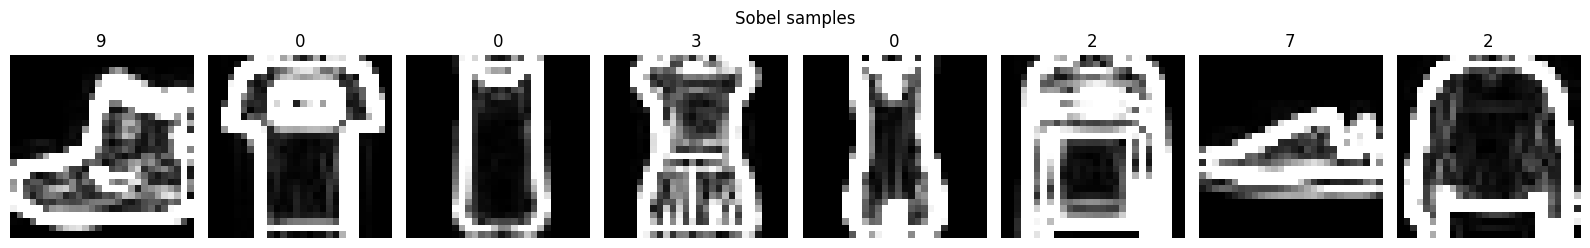
\includegraphics[width=0.8\linewidth]{ann_fashion_sobel_samples.png}
    \caption{Ví dụ ảnh Fashion MNIST sau Sobel}
    \label{fig:fashion-sobel-samples}
\end{figure}

\begin{figure}[H]
    \centering
    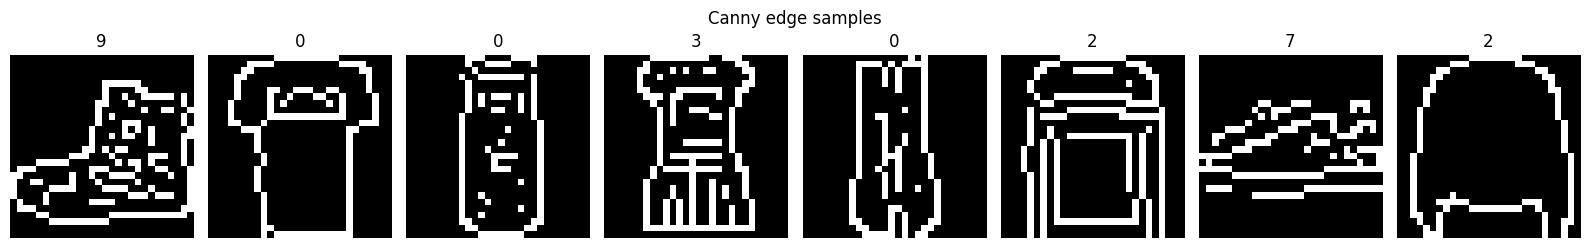
\includegraphics[width=0.9\linewidth]{ann_fashion_canny_samples.png}
    \caption{Ví dụ ảnh Fashion MNIST sau Canny (biên gắt, mất thông tin nội dung)}
    \label{fig:fashion-canny-samples}
\end{figure}

\textbf{Cải tiến 2: Chiến lược huấn luyện}
\begin{itemize}
    \item Ap dung cho mo hinh raw pixels (khong feature engineering), fine-tune theo hai giai doan: train backbone, tang cuong du lieu voi learning rate nho, roi train lai du lieu goc.
    \item Kết quả: Accuracy 0.9031 (F1 0.9031), cao hơn baseline nhưng vẫn thấp hơn HOG.
\end{itemize}

\begin{figure}[H]
    \centering
    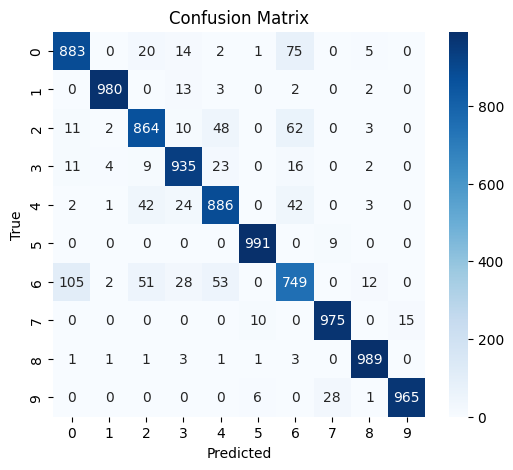
\includegraphics[width=0.6\linewidth]{ann_confusion_matrix_best_fashion.png}
    \caption{Ma trận nhầm lẫn của mô hình tốt nhất cho Fashion MNIST}
    \label{fig:fashion-cm-best}
\end{figure}

\subsection{PneumoniaMNIST}
\textbf{Bảng tổng hợp cải tiến (từ notebook clean)}
\begin{table}[H]
    \centering
    \caption{Kết quả các cải tiến trên PneumoniaMNIST}
    \label{tab:pneumonia-improvements}
    \begin{tabular}{lrrrr}
        \toprule
        \textbf{Phương pháp} & \textbf{Accuracy} & \textbf{F1} & \textbf{Precision} & \textbf{Recall} \\
        \midrule
        Raw & 0.8878 & 0.8883 & 0.8896 & 0.8878 \\
        Augmentation & 0.8446 & 0.8346 & 0.8667 & 0.8446 \\
        HOG & 0.8958 & 0.8927 & 0.9035 & 0.8958 \\
        CLAHE & 0.8157 & 0.7980 & 0.8553 & 0.8157 \\
        CLAHE + HOG & 0.8253 & 0.8153 & 0.8396 & 0.8253 \\
        Weighted Loss & 0.8894 & 0.8855 & 0.8992 & 0.8894 \\
        HOG + Weighted Loss & 0.8942 & 0.8914 & 0.8998 & 0.8942 \\
        \bottomrule
    \end{tabular}
\end{table}

\textbf{Nhận xét chính}
\begin{itemize}
    \item HOG là cải tiến tốt nhất theo Accuracy trong các thử nghiệm ở notebook clean (0.8958).\footnote{skimage.feature.hog: \href{https://scikit-image.org/docs/stable/api/skimage.feature.html\#skimage.feature.hog}{https://scikit-image.org/docs/stable/api/skimage.feature.html}}
    \item Weighted loss giúp cân bằng Precision/Recall; kết hợp HOG + weighted loss cho kết quả ổn định và gần với HOG thuần.
    \item CLAHE và CLAHE + HOG không mang lại cải thiện rõ do nhiễu tương phản cục bộ.
\end{itemize}

\begin{figure}[H]
    \centering
    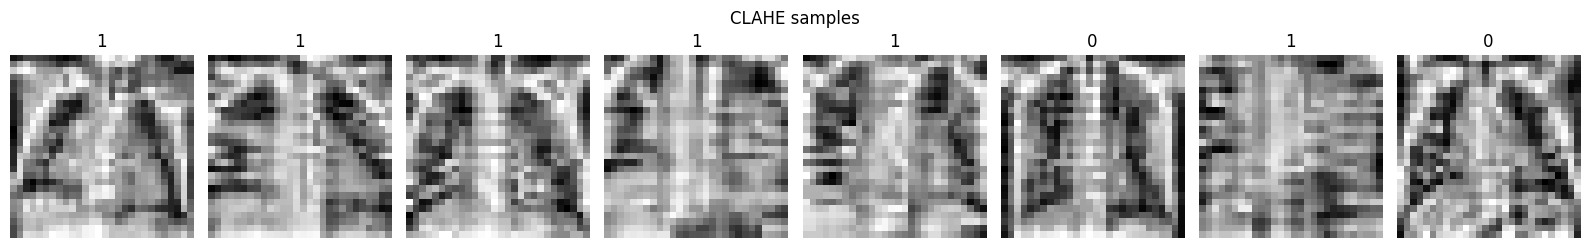
\includegraphics[width=0.9\linewidth]{ann_med_contrast_clahe_samples.png}
    \caption{Ví dụ ảnh PneumoniaMNIST sau CLAHE}
    \label{fig:med-clahe-samples}
\end{figure}

\begin{figure}[H]
    \centering
    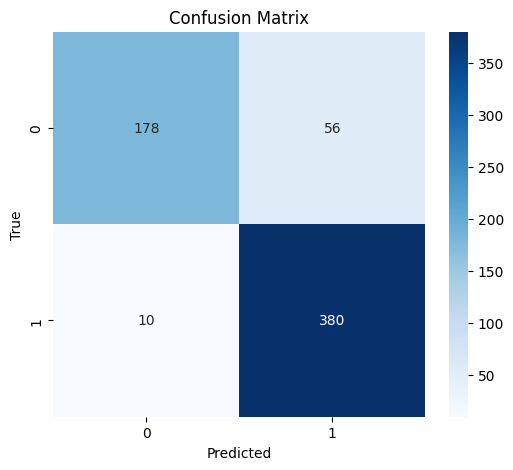
\includegraphics[width=0.55\linewidth]{ann_confusion_matrix_best_med.png}
    \caption{Ma trận nhầm lẫn của mô hình tốt nhất cho PneumoniaMNIST}
    \label{fig:med-cm-best}
\end{figure}

\section{So sánh kết quả}
\subsection{Bảng tổng hợp}
\begin{table}[H]
    \centering
    \caption{So sánh baseline và cải tiến tốt nhất theo Accuracy}
    \label{tab:compare-best}
    \begin{tabular}{lrr}
        \toprule
        \textbf{Dataset} & \textbf{Baseline Acc} & \textbf{Best Acc} \\
        \midrule
        Digit MNIST & 0.9438 & 0.9939 \\
        Fashion MNIST & 0.8443 & 0.9221 \\
        PneumoniaMNIST & 0.8878 & 0.8958 \\
        \bottomrule
    \end{tabular}
\end{table}

\subsection{Phân tích}
HOG giúp tăng mạnh ở Digit và Fashion vì đặc trưng biên/hình dạng rõ rệt. Với PneumoniaMNIST, HOG và HOG + weighted loss cho kết quả gần nhau; weighted loss hữu ích để cân bằng Precision/Recall trong bối cảnh lệch lớp. Augmentation hữu ích khi dữ liệu đa dạng hình dạng, nhưng hiệu quả phụ thuộc đặc trưng và chiến lược huấn luyện.

\section{Kết luận}
\begin{itemize}
    \item ANN phù hợp nhất với Digit MNIST, khá tốt với Fashion MNIST, và hạn chế với PneumoniaMNIST do texture phức tạp và mất cân bằng lớp.
    \item Giới hạn chính của ANN là mất thông tin không gian khi flatten và nhạy với mất cân bằng lớp.
    \item Hướng mở rộng: dùng CNN, tăng cường dữ liệu có kiểm soát, weighted loss/metrics theo lớp, và thử mô hình học đặc trưng chuyên sâu cho ảnh y khoa.
\end{itemize}

\end{document}